\documentclass[12pt]{article}
\usepackage[T1]{fontenc}
\usepackage[fleqn]{amsmath}
\usepackage{amssymb,amsfonts,amsthm,textcomp,mathrsfs}
\usepackage[subfigure]{tocloft}
\usepackage[hang]{subfigure}
\usepackage[title,titletoc]{appendix}
\usepackage{array}
\usepackage[pdftex]{graphicx}
\usepackage{grffile}
\usepackage{rotating}
\usepackage[usenames]{color}
\usepackage{tabularx,supertabular}
\usepackage{multirow}
\usepackage{hhline}
\usepackage{fancyhdr}
\usepackage{natbib}
\usepackage{vruler}
\usepackage{sectsty}
\usepackage{ctable}
\usepackage[utf8]{inputenc}

\usepackage{hyperref}
\usepackage[
    open,
    openlevel=2,
    atend
]{bookmark}[2011/12/02]

\allsectionsfont{\normalsize\bfseries}
\renewcommand{\cftsecfont}{\normalfont}
\renewcommand{\cftsecleader}{\cftdotfill{\cftdotsep}}
\renewcommand{\cftsecpagefont}{\normalfont}

\renewcommand\rmdefault{ptm}
\hypersetup{colorlinks=true, linkcolor=black, citecolor=black, filecolor=black, urlcolor=black, pdftitle=Thesis Title, pdfauthor=Author Name, pdfsubject=, pdfkeywords={text1} {text2} {text3}, pdfcreator=, pdfproducer=}

\newcommand\textstyleJournalNames[1]{\foreignlanguage{english}{\textrm{\textmd{\textit{#1}}}}}

\setcounter{secnumdepth}{3}
\newcommand\mysection[1]{\vspace*{-0.35cm}\section{#1}\vspace*{6pt}\thispagestyle{empty}}
\newcommand\mysubsection[1]{\subsection{#1}}
\newcommand\mysubsubsection[1]{\subsubsection{#1}}

\newtheorem{thm}{Theorem}[section]
\newtheorem{cor}[thm]{Corollary}
\newtheorem{lem}[thm]{Lemma}
\newtheorem{defin}[thm]{Definition}

\makeatletter
\newcommand\arraybslash{\let\\\@arraycr}
\makeatother

\newcommand\liststyleLi{
\renewcommand\labelitemi{${\bullet}$}
\renewcommand\labelitemii{${\circ}$}
\renewcommand\labelitemiii{${\blacksquare}$}
\renewcommand\labelitemiv{${\bullet}$}
}

\setlength\paperwidth{21cm}
\setlength\paperheight{29.7cm}
\setlength\voffset{-1in} %printer
\setlength\hoffset{-1in} %printer
\setlength\topmargin{1.5cm}
\setlength\oddsidemargin{3.5cm}
\setlength\textheight{23.7cm}
\setlength\textwidth{15cm}
\setlength\marginparsep{0cm}
\setlength\marginparwidth{0cm}
\setlength\footskip{1.1cm} %printer
\setlength\headheight{0,6cm}
\setlength\headsep{1,4cm}

\makeatletter
\newcommand\ps@Standard{
  \renewcommand\@oddhead{}
  \renewcommand\@evenhead{}
  \renewcommand\@oddfoot{}
  \renewcommand\@evenfoot{}
  \renewcommand\thepage{\arabic{page}}
}
\makeatother

\pagestyle{fancy}
\renewcommand{\headrulewidth}{0pt}
\renewcommand{\footrulewidth}{0pt}
\fancyhead{}
\fancyfoot{}

\setlength\tabcolsep{1mm}
\renewcommand\arraystretch{1}

\makeatletter
\newcommand\captionof[1]{\def\@captype{#1}\caption}
\makeatother

\newcounter{MathFormule}[section]
\renewcommand\theMathFormule{\thesection \arabic{MathFormule}}
\renewcommand{\baselinestretch}{1.5}
\setlength{\parskip}{\baselineskip}
\setlength{\parindent}{0mm}
\setlength{\tabcolsep}{1pt}

\newenvironment{mytableenv}
{\setlength{\abovecaptionskip}{24pt}
\setlength{\belowcaptionskip}{-18pt}
\centering}
{\setlength{\abovecaptionskip}{0pt}
\setlength{\belowcaptionskip}{0pt}
\par}

\newenvironment{myfigureenv}
{\setlength{\abovecaptionskip}{-6pt}
\setlength{\belowcaptionskip}{24pt}
\centering}
{\setlength{\abovecaptionskip}{0pt}
\setlength{\belowcaptionskip}{0pt}
\par}

\setlength\jot{6pt}
\renewcommand{\theequation}{\thesection \arabic{equation}}
\numberwithin{equation}{section}
\numberwithin{figure}{section}
\numberwithin{table}{section}

\hyphenpenalty=500

\newcommand\mathspaceadjust{
\vspace{6mm}
\topsep=0pt
\partopsep=0pt
\abovedisplayskip=0pt
\abovedisplayshortskip=0pt
\belowdisplayskip=0pt
\belowdisplayshortskip=0pt
}
\mathspaceadjust

\title{}

\begin{document}

%\clearpage
\setcounter{page}{1}
\pagenumbering{roman}
\cfoot{\roman{page}}
\thispagestyle{empty}
{
\vspace*{-14mm}
\centering\textbf{TITLE}\\\vspace*{1.5mm}
\centering\textbf{TITLE CONT.}\\\vspace*{1.5mm}
\centering{(TITLE IN TURKISH)}\\\vspace*{1.5mm}
\vspace*{15.5mm}
\centering{by}\\\vspace*{1.5mm}
\centering\textbf{AUTHOR NAME, M.S.}\\
\vspace*{30pt}
\centering\textbf{Thesis}\\\vspace*{1.5mm}
\centering{Submitted in Partial Fulfillment}\\\vspace*{1.5mm}
\centering{of the Requirements}\\\vspace*{1.5mm}
\centering{for the Degree of}\\
\vspace*{30pt}
\centering\textbf{DOCTOR OF PHILOSOPHY}\\\vspace*{1.5mm}
\centering{in}\\\vspace*{1.5mm}
\centering\textbf{INDUSTRIAL ENGINEERING}\\\vspace*{1.5mm}
\centering{in the}\\\vspace*{1.5mm}
\centering\textbf{INSTITUTE OF SCIENCE AND EGINEERING}\\\vspace*{1.5mm}
\centering{of}\\\vspace*{1.5mm}
\centering\textbf{GALATASARAY UNIVERSITY}\\
\vspace*{30pt}
\centering{Supervisor: Assoc. Prof. Dr. Name}\\\vspace*{1.5mm}
\vspace*{28.5mm}
\centering{Month Year}\\
}

\clearpage
\setcounter{page}{1}
\pagenumbering{roman}
\cfoot{\roman{page}}
\thispagestyle{empty}
{
\vspace*{-7.5mm}
\centering\textbf{TITLE}\\\vspace*{1.5mm}
\centering\textbf{TITLE CONT.}\\\vspace*{1.5mm}
\centering{(TITLE IN TURKISH)}\\\vspace*{1.5mm}
\vspace*{13mm}
\centering{by}\\\vspace*{1.5mm}
\centering\textbf{Ozan ÇAĞLAYAN, B.S.}\\
\vspace*{30pt}
\centering\textbf{Thesis}\\\vspace*{1.5mm}
\centering{Submitted in Partial Fulfillment}\\\vspace*{1.5mm}
\centering{of the Requirements}\\\vspace*{1.5mm}
\centering{for the Degree of}\\
\vspace*{30pt}
\centering\textbf{MASTER OF SCIENCE}\\\vspace*{1.5mm}
\centering{in}\\\vspace*{1.5mm}
\centering\textbf{COMPUTER ENGINEERING}\\\vspace*{1.5mm}
\centering{in the}\\\vspace*{1.5mm}
\centering\textbf{INSTITUTE OF SCIENCE AND ENGINEERING}\\\vspace*{1.5mm}
\centering{of}\\\vspace*{1.5mm}
\centering\textbf{GALATASARAY UNIVERSITY}\\
\vspace*{60pt}
\vspace*{16.5mm} %printer
\centering{February 2014}\\
}

\clearpage
\setcounter{page}{1}
\pagenumbering{roman}
\cfoot{\roman{page}}
\thispagestyle{empty}
{
\vspace*{-7.5mm}
\centering\textbf{A PORTABLE AND EMBEDDED SSVEP BCI SYSTEM: emBCI}\\\vspace*{1.5mm}
\centering{(TAŞINABİLİR VE GÖMÜLÜ BİR SSVEP BBA SİSTEMİ: emBCI)}\\\vspace*{1.5mm}
\vspace*{13mm}
\centering{by}\\\vspace*{1.5mm}
\centering\textbf{Ozan ÇAĞLAYAN, B.S.}\\
\vspace*{30pt}
\centering\textbf{Thesis}\\\vspace*{1.5mm}
\centering{Submitted in Partial Fulfillment}\\\vspace*{1.5mm}
\centering{of the Requirements}\\\vspace*{1.5mm}
\centering{for the Degree of}\\
\vspace*{30pt}
\centering\textbf{MASTER OF SCIENCE}\\
\vspace*{10pt}
\begin{alignat*}{2}
 & \quad\quad\quad\quad\quad\text{Date of Submission \quad } && \text{: January 3, 2014} \\
 & \quad\quad\quad\quad\quad\text{Date of Defense Examination \quad } && \text{: January 27, 2014}
\end{alignat*}
\vspace*{10pt}
\begin{alignat*}{2}
 & \text{Supervisor} && \text{: Assist. Prof. Dr. R. Burak ARSLAN} \\
 & \text{Committee Members \quad } && \text{: Assoc. Prof. Dr. S. Emre ALPTEKİN} \\
 & \text{} && \text{\; Assist. Prof. Dr. B. Atay ÖZGÖVDE}
\end{alignat*}
}

%%%%%%%%%%%%%%%%%%%%%%
%% ACKNOWLEDGEMENTS %%
%%%%%%%%%%%%%%%%%%%%%%
\clearpage
\vspace*{-0.35cm}
\section*{Acknowledgements}
\addcontentsline{toc}{section}{Acknowledgements}
\vspace*{6pt}
\par{
Back in 2007, I remember how I was fascinated when I had heard about Brain-computer interfaces.
}
\par{
Last but not least, I would like to thank my family and my friends for supporting me throughout my life.
}
\par{
Finally, I would like to dedicate this thesis to Ethem Sarısülük, Mehmet Ayvalıtaş, Abdullah Cömert, Medeni Yıldırım, Ali İsmail Korkmaz,
Ahmet Atakan and Hasan Ferit Gedik who passed away during \em{Gezi Unrest}.\\
"Our hearts shall wither if we ever forget."
}

\vspace*{2cm}
\begin{flushright}
February 2014, Istanbul \\
Ozan Çağlayan
\end{flushright}
\clearpage

%%%%%%%%%%%%%%%%%%%%%%%
%% TABLE OF CONTENTS %%
%%%%%%%%%%%%%%%%%%%%%%%
\setcounter{tocdepth}{5}
\renewcommand\contentsname{\normalsize\bfseries Table of Contents}
\phantomsection
\thispagestyle{empty}
\vspace*{0.15cm}
\addcontentsline{toc}{section}{Table of Contents}
\tableofcontents
\clearpage

%%%%%%%%%%%%%%%%%%%%%
%% LIST OF SYMBOLS %%
%%%%%%%%%%%%%%%%%%%%%
\vspace*{-0.35cm}
\thispagestyle{empty}
\section*{List of Symbols}
\addcontentsline{toc}{section}{List of Symbols}
Some text...
\vspace*{6pt}
\clearpage

%%%%%%%%%%%%%%%%%%%%%
%% LIST OF FIGURES %%
%%%%%%%%%%%%%%%%%%%%%
\renewcommand\listfigurename{\normalsize\bfseries List of Figures}
\phantomsection
\thispagestyle{empty}
\vspace*{0.15cm}
\addcontentsline{toc}{section}{List of Figures}
\listoffigures
\clearpage

%%%%%%%%%%%%%%%%%%%%
%% LIST OF TABLES %%
%%%%%%%%%%%%%%%%%%%%
\renewcommand\listtablename{\normalsize\bfseries List of Tables}
\phantomsection
\thispagestyle{empty}
\vspace*{0.15cm}
\addcontentsline{toc}{section}{List of Tables}
\listoftables
\clearpage

%%%%%%%%%%%%%%
%% ABSTRACT %%
%%%%%%%%%%%%%%
\vspace*{-0.35cm}
\thispagestyle{empty}
\section*{Abstract}
\addcontentsline{toc}{section}{Abstract}
\vspace*{6pt}

\par{
Abstract abstract abstract.
}
\clearpage

%%%%%%%%%%%%
%% RESUME %%
%%%%%%%%%%%%
\vspace*{-0.35cm}
\thispagestyle{empty}
\section*{R\'{e}sum\'{e}}
\addcontentsline{toc}{section}{R\'{e}sum\'{e}}
\vspace*{6pt}

\par{
Resume resume resume.
}
\clearpage

%%%%%%%%%%
%% OZET %%
%%%%%%%%%%
\vspace*{-0.35cm}
\thispagestyle{empty}
\section*{\"{O}zet}
\addcontentsline{toc}{section}{\"{O}zet}
\vspace*{6pt}

\par{
Ozet ozet ozet.
}
\clearpage

%%%%%%%%%%%%%%%%%%
%% INTRODUCTION %%
%%%%%%%%%%%%%%%%%%
\mysection{INTRODUCTION}
\thispagestyle{fancy}
\pagenumbering{arabic}
\chead{\arabic{page}}
\cfoot{}
\par{
The objective of a brain-computer interface is to provide an alternative way of interaction between the brain and the environment
without the involvement of muscular pathways. Besides being a revolutionary human computer interface for gaming and entertainment,
BCIs constitute the only way of interaction/communication with the outer world for people who cannot voluntarily control/move their muscles.
}
\par {
Electroencephalography is a non-invasive method for measuring the electrical activity generated within the brain structures, through the scalp.
Although an electrode placed on the scalp measures a linear mixture of various electrical sources underlying the electrode site, 
we can deduce some informations from those measurements using various signal processing and pattern recognition techniques.
}
\clearpage

%%%%%%%%%%%%%%%%%%
%% SECTION: BCI %%
%%%%%%%%%%%%%%%%%%
\mysection{BRAIN COMPUTER INTERFACES}\label{seq:bci}

\par{
    The locked-in syndrome (LIS) is a medical condition in which patients are awake and conscious but 
    cannot move or communicate verbally because of complete paralysis of nearly all voluntary muscles. 
    LIS is mostly caused by traumatic brain injuries, brain strokes, hemorrhages, head trauma, demyelinating diseases 
    or infectious conditions.
}

% LIS classification

\par {
    Amyotrophic Lateral Sclerosis (ALS), also known as Lou Gehrig's disease (Lou Gehrig is a popular baseball 
    player who was diagnosed with ALS in 1939) is another disease leading to LIS. ALS basically attacks 
    motor neurons that control voluntary muscles in the body. When those motor neurons stops functioning, 
    the muscles lose strength and progressively die (Atrophy).
}

\par {
    According to ALS Association, nearly 5600 people in the United States are 
    diagnosed with ALS each year and the incidence of the disease is 2 per 100.000 
    people\footnote{\url{http://www.alsa.org/about-als/facts-you-should-know.html}}.
}

\par{
    When consciousness and cortical functions are preserved, it may actually be 
    possible to use healthy brain activity in order to build a novel way of interaction 
    between the subject's brain and the environment using special brain signal 
    acquisition techniques and computers. These composite systems are called 
    Brain-Computer Interfaces (BCI) or Brain-Machine Interfaces (BMI).
}

\mysubsection{Definition}\label{seq:bci_definition}
\mysubsection{Objective and Motivation}\label{seq:bci_motivation}
\mysubsection{History}\label{seq:bci_history}
\mysubsection{Principles}\label{seq:bci_principles}
\par{
Parts of the brain (visual, auditory, vs, resim), linear mixture of sources, belki biraz source localization, 
}

% EEG, ECoG, Intracortical, MEG, fMRI, NIRS
\mysubsection{Signal Acquisition Methods}\label{seq:bci_methods}
\mysubsubsection{EEG}\label{seq:bci_methods_eeg}
\mysubsubsection{ECoG}\label{seq:bci_methods_ecog}
\mysubsubsection{Intracortical Recordings}\label{seq:bci_methods_intracortical}
\mysubsubsection{fMRI}\label{seq:bci_methods_fmri}
\mysubsubsection{fNIRS}\label{seq:bci_methods_fnirs}


% EEG based BCIs
\mysubsection{EEG based BCIs}\label{seq:eeg_bci}
\mysubsubsection{Montage and Recording}\label{seq:eeg_recording}
\par{
10-20 setup (resim), electrode naming (tek, cift), bipolar-unipolar recordings, referencing, 
electrode types (aktif, pasif, jel, dry, resim)
}

%%%%%%%%%%%%%
%% SECTION %%
%%%%%%%%%%%%%
\clearpage
\vspace*{-0.35cm}
\mysection{HARDWARE}\label{seq:hardware}

\mysubsection{Why Embedded Computer?}\label{seq:embeddedcomputer}

\par{
Single computer BCIs generally require decent computers as they can make use of heavy signal processing 
and machine learning algorithms while probably presenting visual stimuli in a precise timing.
}

\par{
Today, the embedded computers found on smartphones are much powerful compared to the desktop PCs 
used in the BCI systems designed years ago. The main concern of this study is to assess whether small, 
(possibly) battery-powered and cheap embedded computers can be used to replace big, power hungry and 
expensive computers in a simple, online BCI system.
}

\mysubsubsection{Advantages}\label{seq:embeddedcomputer_advantages}

\par{
Majority of embedded computers runs Linux which does not require a graphical desktop environment 
to be available. This allows to reduce memory and CPU usage on these systems as the most resource 
hungry component of a modern operating systems is the Graphical User Interface (GUI).
}

\par{
Using Linux also helps to prepare a custom OS designed to run the BCI loop efficiently. 
This is achieved by removing/disabling system services and applications which won't be required at all by BCIs.
}

\par{
All of these optimizations reduce the overall power consumption of the embedded BCI which brings 
the possibility to use a battery-pack as power supply. This final achievement is key to ultimate 
portability of BCI systems.
}

\mysubsection{BeagleBone Black}\label{seq:embeddedcomputer_bbb}

\par{
BeagleBone Black (BBB) (Figure ~\ref{fig:bbb}) is a 45\$ single board computer released in 2013. It has 1GHz TI AM3359 Sitara ARM Cortex-A8 microprocessor, 
512MB DDR3 memory, 3D accelerated PowerVR SGX530 graphical processing unit (GPU) with HDMI output, onboard 2GB embedded MMC (eMMC) 
flash storage pre-loaded with Ångström Linux distribution. Along with a single USB 2.0 host port and 10/100 RJ45 Ethernet port for general purpose connectivity, the board also provides a wide variety of low-level expansion interfaces: 
4xUART, 8xPWM, 2xSPI, 1xADC and 2xI\textsuperscript{2}C.
}

\begin{figure}[ht]
    \centering
    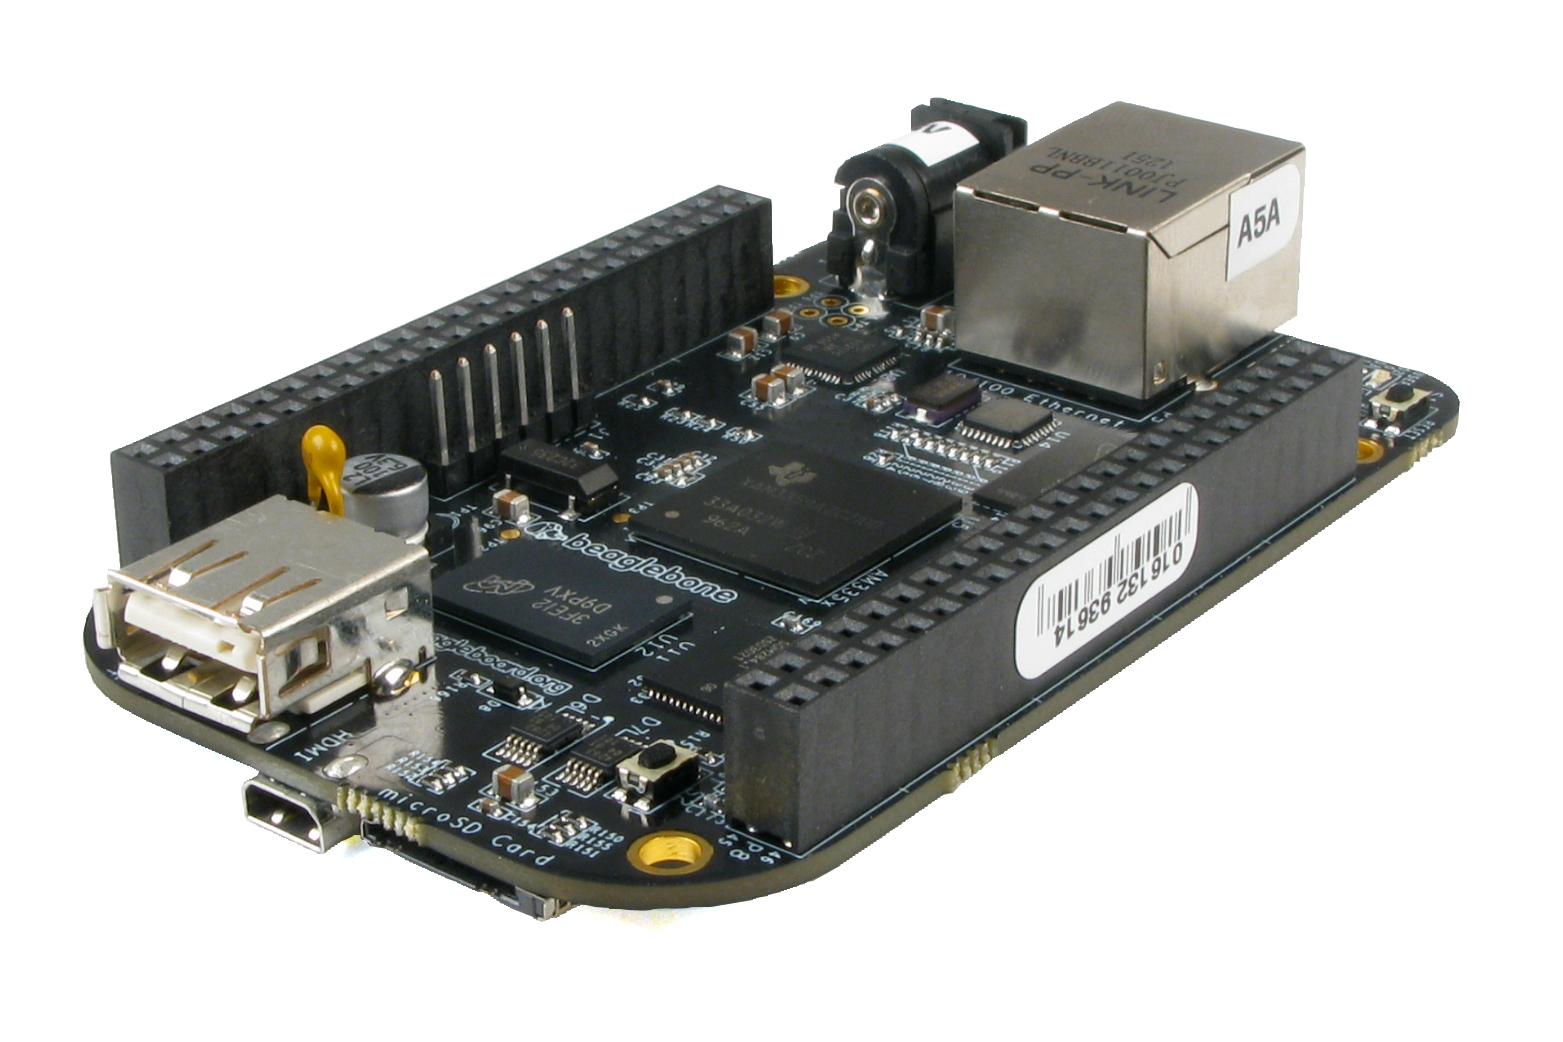
\includegraphics[width=0.4\textwidth]{images/bbb}
    \caption{BeagleBone Black Single-board Computer.}
    \label{fig:bbb}
\end{figure}

\mysubsubsection{Initial Setup and Customization}\label{seq:embeddedcomputer_initialsetup}
\par{
We first installed Ubuntu (into the onboard eMMC storage) as it is a widely adopted Linux distribution with a rich software repository. A rich software repository is important for avoiding 
manual compilation/installation of several tools and libraries, which in turn decreases time needed to start experimenting with the BCI system.
}

\par{
The list of tools and libraries that we'll be frequently using throughout this work are: {\em Git, python-emotiv, SciPy, NumPy, python-bitstring, pycrypto, pyusb, python GPIO library for BBB.}
}

\par{
Several unused system services like BLAH, BLAH, BLAH are completely disabled so that they don't waste available system resources.
}

\mysubsubsection{Stimuli Generation on BBB}\label{seq:embeddedcomputer_stimuligen}
\par{
    BBB has several General-Purpose Input/Output (GPIO) pins that can be used 
    to communicate with external devices and circuits. These pins can be raised 
    HIGH (+3.3v) or LOW (0v) programatically, using GPIO libraries available for 
    Python.
}
\par{
    In order to preserve the portability of the system, we decided to use BBB's 
    GPIO pins for LED SSVEP stimulation instead of a separate/dedicated microcontroller. 
    The wiring of LEDs is quite trivial and can be seen in Figure??.
}

% FIXME: Possible figure for wiring


\mysubsection{Emotiv EPOC EEG}\label{seq:emotivepoceeg}

\par{
    Emotiv EPOC EEG (Figure ~\ref{fig:emotiv_epoc_headset}) is a battery-powered wireless consumer headset which can acquire 14 channels
    of EEG signal. The headset internally applies a notch filter (At line frequency 50/60Hz) and a
    5\textsuperscript{th} order band-pass filter (0.2-45Hz) to the signal. Although the internal sampling rate
    of the headset is 2048Hz, the data packets are delivered to the USB dongle with a rate of 128 samples/second.
    Full technical specifications found in the manufacturer's website\footnote{\url{http://www.emotiv.com/eeg/download_specs.php}} 
    are summarized in Table ~\ref{table:emotiv_epoc_specs}.
}
\par{
Some text \citep{sanei_eeg_2008}...
Some other text \citep{fazli_enhanced_2012}...
}
\begin{figure}[ht]
    \centering
    \includegraphics[width=0.4\textwidth]{images/emotiv}
    \caption{Emotiv EPOC EEG Headset.}
    \label{fig:emotiv_epoc_headset}
\end{figure}

\begin{table}
    \footnotesize
    \centering
    \caption{Technical specifications of Emotiv EPOC EEG.}
    \begin{tabular}{| l | l |}
        \hline
        Number of channels & 14 (+ CMS/DRL references, P3/P4 locations) \\ \hline
        Channel names & AF3, F7, F3, FC5, T7, P7, O1, O2, P8, T8, FC6, F4, F8, AF4 \\ \hline
        Sampling method & Sequential sampling, single ADC \\ \hline
        Sampling rate & 128 SPS (2048 Hz Internal) \\ \hline
        Resolution & 14 bits 1 LSB = 0.51uV \\ \hline
        Bandwidth & 0.2-45Hz, digital notch filters at 50Hz and 60Hz \\ \hline
        Filtering & Built-in digital 5th order Sinc filter \\ \hline
        Dynamic range (input referred) & 8400uV (pp) \\ \hline
        Coupling mode & AC coupled \\ \hline
        Connectivity & Proprietary wireless, 2.4GHz band \\ \hline
        Battery life & 12 hours (typical) \\ \hline
        Impedance measurement & Real-time contact quality using patented system \\ \hline
    \end{tabular}
    \label{table:emotiv_epoc_specs}
\end{table}

\mysubsubsection{Official Software Development Kit (SDK)}\label{seq:emotivepoceeg_sdk}

\par{
Emotiv provides an SDK for Windows, Mac OS X and Linux operating systems but the provided SDK is 
closed-source and only available for x86 CPU architecture. This means that it is not possible 
to use the SDK on ARM embedded computers like Raspberry Pi or Beaglebone Black. 
Currently, the only way of using the EPOC headset with an ARM based embedded computer is to use the 
open-source protocol\footnote{\url{https://github.com/openyou/emokit}} reverse-engineered by Cody Brocious and Kyle Machulis. 
%Stopczynski et al. (2011) developed a mobile brain scanner framework\footnote{\url{https://github.com/SmartphoneBrainScanner}} 
%which runs on Nokia N900 ARM smartphones.
}

\mysubsubsection{Open-Source Protocol}\label{seq:emotivepoceeg_opensource}

\par{
According to the protocol details revealed by the open-source community, 
the USB dongle acts as a simple Human Interface Device (HID) which relays a 
32 bytes AES encrypted data packet with a rate of 128 packets/sec.
}

\par{
Each decrypted packet contains a sequence number to determine lost packets. 
This number ranges from 0 to 127 for raw EEG data. A special sequence number 
128 indicates a status packet which contains battery level and contact 
qualities instead of raw EEG.(The headset reports those status data once in a second.)
}

\par{
Since we decided to develop the BCI in pure Python, we wrote an object oriented 
Python module called \emph{python-emotiv}\footnote{\url{https://github.com/ozancaglayan/python-emotiv}} implementing the open-source protocol to access the device on Linux.
}


%%%%%%%%%%%%%%%%
%% REFERENCES %%
%%%%%%%%%%%%%%%%
\clearpage
\vspace*{-0.35cm}
\bibliographystyle{apalike}
\phantomsection
\thispagestyle{empty}
\addcontentsline{toc}{section}{References}
\bibliography{ThesisLibrary}

%%%%%%%%%%%%%%%%%%%%%%%%%
%% BIOGRAPHICAL SKETCH %%
%%%%%%%%%%%%%%%%%%%%%%%%%
\clearpage
\cfoot{}
\vspace*{-0.35cm}
\thispagestyle{empty}
\section*{Biographical Sketch}
\addcontentsline{toc}{section}{Biographical Sketch}
\vspace*{6pt}
\par{
Ozan Çağlayan was born on September 11, 1985 in Istanbul, Turkey. After graduating from Saint-Joseph French High School in 2004,
he began studying Computer Engineering at Galatasaray University. In 2007, he spent a semester at Université Joseph Fourier (Grenoble/France) as part of Erasmus Exchange Programme.
In September 2007, he became a part-time software developer of Pardus Linux, the national Linux-based operating system project
managed by The Scientific and Technological Research Council of Turkey (TUBITAK). After receiving his Bachelor of Science in 2008, he continued working for Pardus Linux project until January 2012.
Since October 2012, he is working as a research assistant at Galatasaray University.
}
\clearpage

\end{document}
